\begin{savequote}[75mm]
A new life awaits you in the Off-world colonies! A chance to begin again in a golden land of opportunity and adventure!
\qauthor{Blade Runner}
\end{savequote}

\chapter{Online identities as hypermedia documents}

\newthought{Web services} use personal data to sustain their business by fuelling this stream of information to recommendation systems to generate tailored advertising. When users decide to subscribe a service, they automatically lose control over the data generated by their activity. This is especially true when third parties are authorised to access a user's profile and information. 
This chapter is focused on describing how user data is transferred from mobile and web application implementing their login flow through a larger authorisation provider, like Google or Facebook, and how this could be improved. Leveraging on work from~\cite{puglisi2015restful} on open web applications, and continuing on the study from~\cite{puglisi2015potential}, we introduce a hypermedia model of the user online footprint. We show furthermore, how web and mobile app already use hypermedia docuements to handle user data. Ultimately we use an example of a privacy broker to show how existing technologies can be used to allow users to retain control on their data. Our defined model can be both used to transfer data between services and clients and to express the value and risk of sharing certain information.

\section{Background}

The business model of many services and applications on today's web is based on having user authenticate and, completely or partially, generate data to \emph{pay} for the possibility to use the service. Data is, in fact, used as a currency that can be resold for a variety of purposes. To target the users and suggest back product that they can buy, or to continuously track them across different visits, and in some cases different devices and websites.

Web services can furthermore dispose of the data collected as their property, as when users access a service they lose control and rights over their digital footprint. One of the problem associated with this is certainly linked to consent. Users give their implicit consent to the use of their data and subsequently their footprint, sometimes only in part, become property of the company providing the services. The same process of giving consent or granting permissions to access part of the user identity is not clear. This scenario is particularly evident when mobile applications request access to some resources on a user's phone, or when Facebook federated login mechanism is used. Facebook login provides both authentication and authorisation. The mechanism is used on the web as well as on iOS and Android, although on those platforms the primary mechanism uses the native Facebook application instead of the web API. When an application is connected to the user's Facebook profile using Facebook login, it can always access their \emph{public profile} information. Facebook consider this information public and will not apply any restriction on it. Information that is shared with the public profile vary from user to user and depends on their privacy settings. By default, the Facebook public profile includes some basic attributes about the person such as the user's age range, language and country, but also the name, gender, username and user ID (account number), profile picture, cover photo and networks. This is the minimum set of data disclosed by Facebook when the social network login mechanism is used to gain access to an app or service. This data is acquired by the app and user control over it is practically lost, as it will be disposed according to the app privacy policy.
We propose an example scenario of a privacy broker implementing a privacy friendly authentication mechanism. We introduce two particular examples, the first one is based on the WebSocket protocol and shows a handshake based on the Socialist Millionaires protocol. The second example is based on the OAuth 2.0 flow which uses JWT to transmit private information to third parties. This examples builds upon previously published approaches and techniques, such as Crypto-Book~\cite{maheswaran2013crypto} and UnlimitID~\cite{isaakidis2016unlimitid}, using the technique of blacklistable anonymous credentials~\cite{tsang2007blacklistable}. The idea behind these techniques is that a trusted (or semi trusted) Privacy Broker (PB) issues an anonymous credential $C(x)$ encoding a secret identity key x, unique and only known by the specific user. The user holding C(x) authenticates to a Service Provider (SP) by, given a cryptographically secure hash function and a secure elliptic curve group, producing a ticket $T$ depending on $x$, together with a zero-knowledge proof stating that they actually hold a valid credential from the PB, the key used to compute $T$ is the same as their secret identity key used to compute $C(x)$ and no previous ticket associated with past abuses used the identity key $x$. 
The examples proposed are presented to illustrate how a privacy broker could help the user maintain a desired footprint. Furthermore, the examples show how existing web protocols can be used to allow the user to authenticate anonymously to the SP and eventually disclose private information with the same SP or third-parties as they please. We would like to stress that we do not present novel cryptographic protocols, nor we propose modifications for existing web protocols or clients and that we make use of existing and widely adopted authorisation and authentication mechanism. Furthermore, the proposed hypermedia model allows the user to explore the shared preferences and properties shared with each service.

\section{A hypermedia model of the user identity}

Users interact with web services and applications with hypermedia protocols. Each time an action is completed onto an user's phone a call is performed to an APIs updating the user profile or sending some information to a service. These interactions are often completed over a REST protocol, such as HTTP, and consist of the client sending structured information to the server. This information can be anything regarding the user or the state of the used application, such as profile information or answers to specific queries initiated implicitly or explicitly by the user.

We define a model of the user identity to describe how a privacy policy can interact with data and which data or resource a service can access. Our model is based on the assumption that user data can be represented with a hypermedia object. 

The whole concept of hypermedia is about making clients interact better with services, and making resources easily accessible and can be explored. A can be a record in a database, but it can also contain information from other records, or from other databases or applications. A resource is essentially an object acting as a gateway to some stream of information.

If we think for a moment about the evolution of the Internet and the Web, we are witnessing the transformation of a complex system from a platform of interconnected computers, to a platform of interconnected documents, to a platform of interconnected data streams. 

The uniformity of web interfaces as defined by the RESTful architectural paradigms allows the usage of different types of identifiers to request resources in the same context, providing uniform semantics even when the access mechanism used may be different. As a matter of fact, we don't even have to be concerned with the access mechanism; we just need to ensure that our API replies consistently. The same principles permit us to introduce new types of resource identifiers without having to change the way existing identifiers work, while also allowing reuse of identifiers in a different context.

Building on the principles of RESTful resources, we begin by defining the identity model using JSONApi~\cite{Jsonapi} a specification for exchanging data between REST interfaces. JSONApi can be used to define how a client should request that resources or their representations be fetched or modified, and how a server should respond to those requests. We envision that the same format can be used on the client side to represent identities and data associated with it and on the server side to request and exchange data.

\lstset{caption={Some user identity data encoded with JSONApi.},label=lst:JSONIdentity}
\begin{lstlisting}
{
    "data": {
        "type": "identity",
        "id": "john@johnsmith.com",
        "attributes":
            { // Attribute list },
        "relationships":
                { // Relationship list },
        "links": { // Third-party links }
    },
    "included": [ {
        "type": "resource",
        "id": "CC76598TDZKG9EEC3", // Device hardware id
        "attributes": { // resource attributes }
        "meta": { // Any meta information },
    }],
}
\end{lstlisting}

We model the user's activity as series of events belonging to a certain identity. Each event is a document containing different information. We can formally define this an hypermedia document i.e. an object possibly containing graphics, audio, video, plain text and hyperlinks. We call the hyperlinks selectors and we use these to build the connections between the user's different identities or events. Each identity is a profile that the user has created onto a service or platform. This can be an application account or a social network account, such as their LinkedIn or Facebook unique IDs.

This is consistent with the versatility of RESTful interfaces. In fact, the interesting aspect of REST is that by combining relatively simple architectural elements it is possible to build entire systems with complex functions.

In our hypermedia model, each event is the result of the user performing an action. For the purpose of this study we have consider an action as resulting using an application or a service. An action is the activity of interacting with a mobile application or \emph{liking} a resource on a social network, i.e. directly expressing an interest, or the fact that a user has updated their location at a certain time.

We find that this model is able to express the user's online footprint as a collection of traces left across different services. Furthermore, by using a hypermedia approach we are able to grasp the connections between the different profiles and features. This results in the possibility to profile users based on chosen selectors. For example, we might want to trace all users who have been in the radius of 500 meters to a certain location, or all the users in a certain neighbourhood who \emph{like} a selected Facebook page.

A service implementing the described model of the user identity can either be an identity provider or a client storing user's preferences and data. For example, a user might decide to login to third-party services through a trusted, or semi-trusted, identity provider, allowing them to disclose only a partial representation of their online footprint. The same user might store the full representation of their data locally on their devices or on different services.

The flexibility of this model allow the possibility to develop client applications that can retrieve different snippets of data from different identity providers and disclose information at the user control. We will know discuss how this can be achieved by showing how this can be implemented in well-used authentication protocols.

\section{Data flow between identity providers and third-party services}

At the time of writing, when third-party services use identity providers, like Facebook or Google, for federated login, a number of private data is transferred to the service at the time of login. If we observe a mobile app making a request to Facebook to allow a user to login, we will see how the first call in the process is a OAuth request sending an authorization token as in Listing~\ref{lst:FBRequest}.

\lstset{caption={OAuth request to Facebook.},label=lst:FBRequest}
\begin{lstlisting}
--3i2ndDfv2rTHiSisAbouNdArYfORhtTPEefj3q2f
Content-Disposition: form-data; name="batch_app_id"

464894686855067
--3i2ndDfv2rTHiSisAbouNdArYfORhtTPEefj3q2f
Content-Disposition: form-data; name="batch"

[{"relative_url":"oauth\/access_token?fields=&format=json&grant_type=fb_extend_sso_token&include_headers=false&sdk=ios","method":"GET"},{"relative_url":"me\/permissions?fields=&format=json&include_headers=false&sdk=ios","method":"GET"}]
\end{lstlisting}

If the request is successful, the user is granted permission to use the app and the service is transferred the user's data and authorised to refresh the user information unless this decides to prevent the app from doing so. This authorization is encoded with a \emph{permission: property, status: value} JSON schema. 

\lstset{caption={OAuth response from Facebook to third-party app.},label=lst:FBResponse}
\begin{lstlisting}
[{"code":200,"body":"{\"data\":[{\"permission\":\"user_birthday\",\"status\":\"granted\"},{\"permission\":\"user_relationship_details\",\"status\":\"granted\"},{\"permission\":\"user_likes\",\"status\":\"granted\"},{\"permission\":\"user_education_history\",\"status\":\"granted\"},{\"permission\":\"user_work_history\",\"status\":\"granted\"},{\"permission\":\"user_photos\",\"status\":\"granted\"},{\"permission\":\"user_friends\",\"status\":\"granted\"},{\"permission\":\"user_about_me\",\"status\":\"granted\"},{\"permission\":\"email\",\"status\":\"granted\"},{\"permission\":\"public_profile\",\"status\":\"granted\"}]}"}]
\end{lstlisting}

At this point some services will use the information obtained to compute a user profile that reflects user generated data on their platform and their social identities. An example is a social app including the user's photo feed, as in Listing~\ref{lst:TUProfile}.

\lstset{caption={Example of user profile including user's photos from other apps.},label=lst:TUProfile}
\begin{lstlisting}
"user": {
    "_id": "531e1adefb3c64ad0500b2e5",
    "badges": [],
    "birth_date": "1985-04-27T08:36:13.695Z",                
    "common_connections": [],
    "common_likes": [],
    "distance_mi": 2,
    "gender": 1,
    "group_matched": false,
    "instagram": {
        "completed_initial_fetch": true,
        "last_fetch_time": "2017-04-23T21:25:58.720Z",
        "media_count": 373,
        "photos": [
            {
                "image": "https://scontent.cdninstagram.com/t51.2885-15/34161997201408_n.jpg",
                "link": "https://www.instagram.com/p/BTPi20-AZEU/",
                "thumbnail": "https://scontent.cdninstagram.com/t51.2885-15/s150x150/e35/c18.jpg",
                "ts": "1492982755"
            },
        ...]
    }
}
\end{lstlisting}

Even if the user deletes the app from their phone, the app will maintain the possibility to access their data on the identity provider, unless they will make the effort to delete it also from the list of authorised app. The process is not straightforward, and ultimately the app should request the user permission to access their data instead of obtaining refreshed information from the identity provider.

\section{Mitigation possibilities}

We now discuss through two different examples, a mechanism that would be able to give users more control over their data and desired footprint, given the hypermedia model proposed above. We propose two possible solutions. 
We believe that the main problem with uncontrolled data flow between identity providers and third parties app resides in the way data is transferred when the user accesses the third party service.
The first example uses WebSocket~\cite{fetterfc} to perform a handshake protocol based on the Socialist Millionaires as implemented in Off The Record (OTR) messaging protocol~\cite{goldberg2012off}. The second example uses a known non-interactive Zero-Knowledge proof and is based on the widely adopted Oauth 2.0 protocol~\cite{hardt2012oauth} for authorisation. We describe how JSON Web Token (JWT)~\cite{jones2015json} Bearer can be used for anonymous authorisation and authentication.

\subsection{Describing the OAuth 2.0 example}

\begin{itemize}
    \item Client
    \item Resource Owner
    \item Authorisation Server
    \item Resource Server
\end{itemize}

\begin{figure}
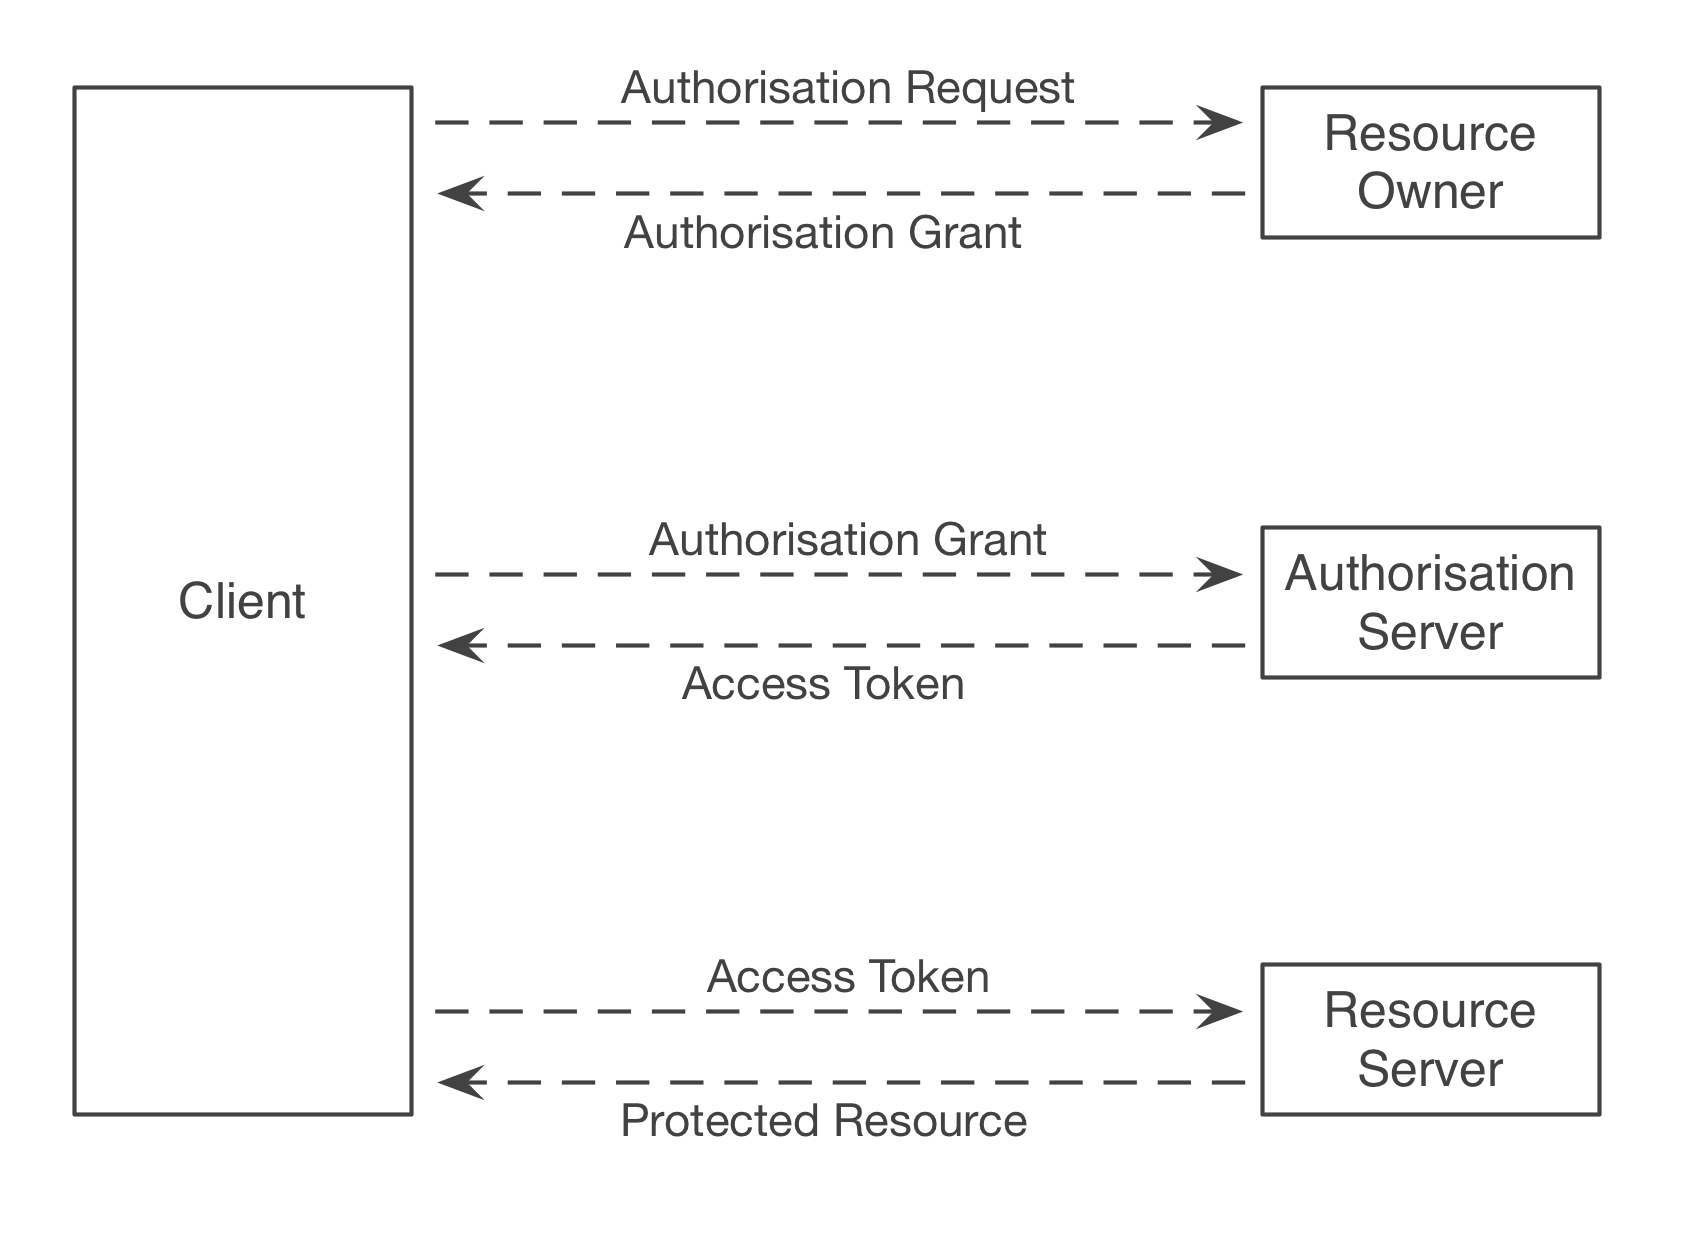
\includegraphics[width=\textwidth]{figures/OAuth2Flow.png}
\caption[OAuth 2.0 Flow.]{The abstract OAuth 2.0 flow describes the interaction between the four roles within the defined steps.
\label{fig:oauth2flow}}
\end{figure}

The six steps in the abstract OAuth 2.0 flow are defined as follows:
\begin{enumerate}
    \item The client sends an authorisation request to the resource owner, either directly or via the authorisation server as intermediary.
    \item The client receives an authorisation grant.
    \item The client requests an access token by presenting the authorisation grant.
    \item The client is authenticated by the authorisation server which issues and access token.
    \item The client now requests the protected resource presenting the access token.
    \item The resource server validates the token and replies with the resource representation if valid.
\end{enumerate}

JSON Web Token (JWT)~\cite{jones2015json} is a compact, URL-safe mechanism to represent and transfer claims between two parties. The claims are encoded as a JSON object. This can be used as the payload of a JSON Web Signature (JWS)~\cite{jones2014n} structure, or as the plaintext in a JSON Web Encryption~\cite{jones2015jwe} structure. Therefore, JWT allows for the claims to be digitally signed or integrity protected integrity protected with a Message Authentication Code (MAC) and/or encrypted.

\subsection{Describing the WebSocket example}

The WebSocket is a protocol created for web application to establish a bi-directional connection between a client running untrusted code and a remote host that has opted-in to communications from that code. 
WebSocket use the common origin-based security model implemented by web browsers, and consists in opening a handshake followed by basic messages framing, layered over TCP.

WebSocket provides a mechanism for browser-based applications to establish a two-way communication with a server without opening multiple HTTP connections based on a handshake protocol, where a WebSocket client or server uses a first a connection upgrade request. If the handshake is successful data can be transferred, by either the client or the server, at will.

Our WebSocket example implements the Socialist Millionaires protocol as used by OTR-chat after the WebSocket handshake and it is used to authenticate the client with the server without having to disclose the user identity.

\subsection{Scenarios}

We consider a scenario in which a user wants to login to a SP without having to directly expose their identity, by leveraging with a chosen privacy broker PB. Both the user and the SP trust the PB to an extent. In this scenario we have three parties:
\begin{itemize}
    \item client
    \item service provider
    \item privacy broker
\end{itemize}

Before starting an authentication and subsequent authorisation process the client needs to create an account with the PB. This step can be consider as an \emph{initialisation} phase.

\subsection{Account creation on the PB}

To create an account on the PB we assume that as the client is initialised it will generate a number of cryptographic keys to authenticate the various user identities. The keys can be saved in a wallet and used to register identities on the PB. A use might decide to use different keys for each service or the same key for a group of services. Note that each key doesn't correspond to a service account Id. A key is actually an account identification for the PB which is stored and used by the client.

To create an account on a service the client prepares a request for the PB performing a set of cryptographic operations that allows the client to register an anonymous identifier for the service. To implement such algorithm, we need a
cryptographically secure hash function and a secure elliptic curve group. JSON Web Algorithms (JWA)~\cite{jones2015jwa}, provides Hash-based Message Authentication Codes (HMACs). HMACs enable the client to compute a MAC from a secret (the user's key) plus a cryptographic hash function. The algorithm for implementing and validating HMACs is provided in RFC 2104~\cite{krawczyk1997rfc}.

The account can be completely anonymous on the PB side as long as the SP is able to eventually blacklist the account in case they perform some malicious action.

\subsection{Authorisation request on OAuth}

A possible OAuth flow can be described as follows (Fig.~\ref{fig:privateflow}):
\begin{enumerate}
    \item The client sends an authorisation request to the PB. This request is signed and encrypted and packed into a JWT.
    \item If the request is valid the PB issues a token.
    \item The client uses the token to authenticate with the service. Which is verified separately with the PB.
    \item The service returns access to the protected resource through its representation.
\end{enumerate}

\begin{figure}
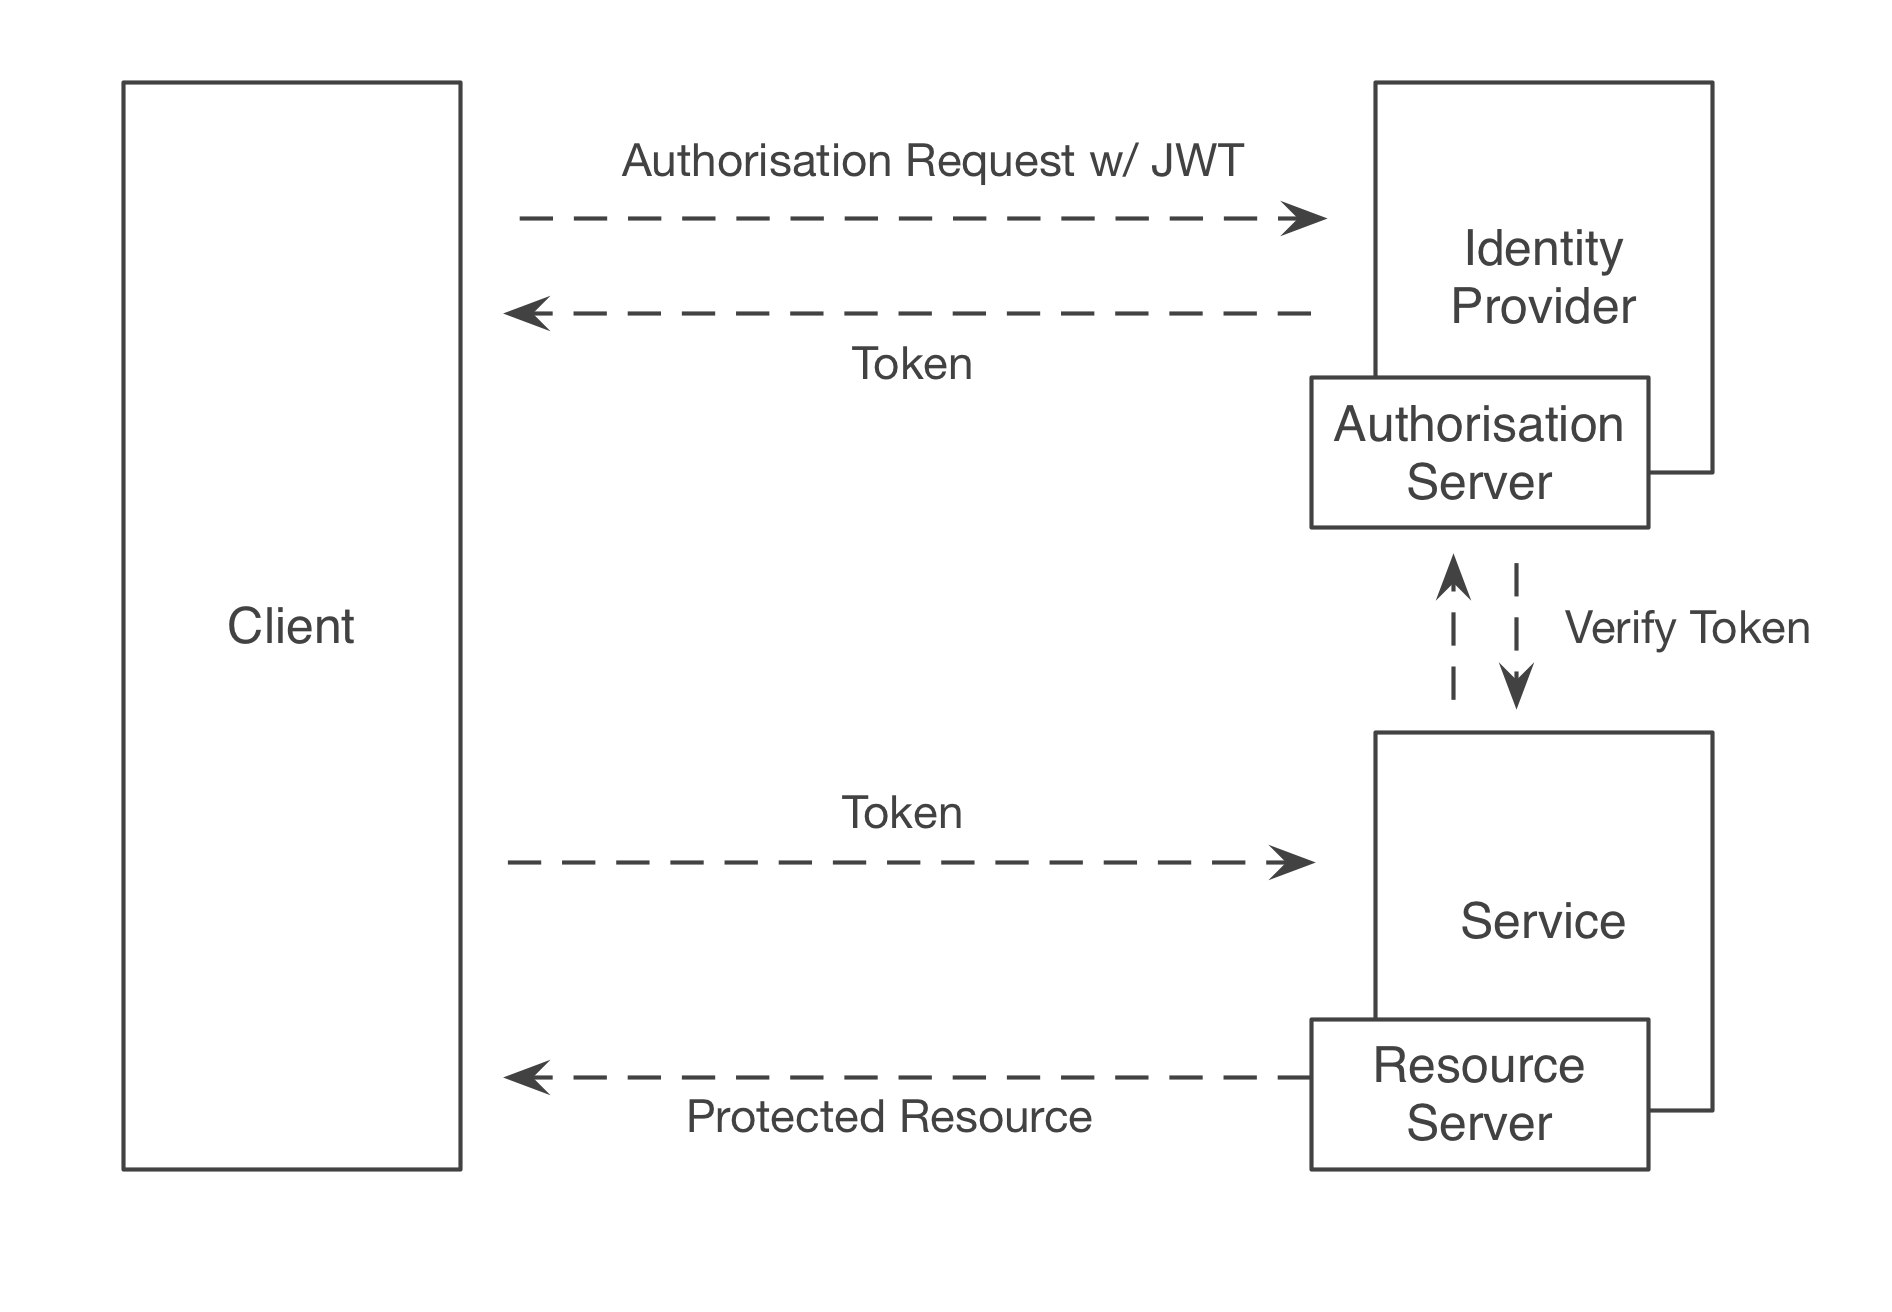
\includegraphics[width=\textwidth]{figures/PrivateFlow.png}
\caption[Privacy Preserving OAuth Flow with JWT.]{The privacy preserving OAuth 2 flow uses JWT to transmit user information.
\label{fig:privateflow}}
\end{figure}

Once the client is issued a \emph{token} from the PB it can authenticate with the \emph{service}. Hence, the issued \emph{token} which encodes the claims and service id can be transmitted to the service encrypted with the JWE protocol. The token can then be verified and the client authorised to request the protected resource. An account is created on the service if the authentication request is initiated for the first time.

The OAuth example was implemented as follows:

\begin{enumerate}
    \item The client sends an authorisation request to the PB.
    \item The client receives an authorisation grant via a \emph{JWT} encoding the 0-knowledge proof to present to the SP.
    \item The client engages the SP in a zero-knowledge proof that it holds a valid credential from the PB.
    \item The client is authenticated (or not).
    \item The client can now request protected resources, or the SP can request further information from the client.
\end{enumerate}

The client can prove to know the secret pseudonym by solving a cryptographic challenge in the request over OAuth to the server and once it is authenticated through the PB can use the obtained OAuth token to communicate with the SP. 

In our example we have considered the client sends the answer to a cryptographic challenge to the server, that can verify the proposed solution and issue a JWT with an authorisation ticket. 

The client can use the ticket to disclose information with the PB or the SP. The PB can use the disclosed information to sing a statement to the SP regarding the client without disclosing the information or can authorise the client to access the SP by vouching for them.

\subsection{Authorisation request on WebSocket}

We imagine that a client has already established a handshake request with a server over WebSocket and is waiting to establish a communication. In this case the client will initiate an authorization process with the server where it wants to prove that it knows the secret pseudonym registered with the server. To prove this, it can initiate a zero-knowledge proof like the Socialist Millionaires protocol to prove the server they know the pseudonym. 
We have used in out example a well-known protocol to show how this could be implemented in practice without having to modify existing web applications logic. Clearly, more efficient protocols and proofs can be used.

An interesting aspect of the WebSocket protocol is that it does provide the possibility to define custom protocols once the first handshake is success full. Here is where the OTR protocol, or another zero-knoledge proof protocol, can be used to preserve client anonymity. 

Once the secure protocol is successful, the client can also initiate the data transfer to disclose information or receive an authorisation ticket that can be used with a third party.

The objective of this example is to show how it is possible to implement a secure protocol on top of existing infrastructure and how this wouldn't affect the mechanism performances nor present a big overhead on the transferred data.

\section{Evaluation}

The examples introduced described up to this point allows the client to granularly disclose information to the SP. More importantly in the current federated log in mechanism, implemented by IdPs like Facebook, third-party apps can always request to the IdP updated information regarding the user. With the proposed mechanism, based on the PB intermediary model, third-party apps will have to request the information to the client, that can refuse to provide them or can provide different values depending on the context. 

A typical scenario is the case for which a user wouldn't like to disclose some of their preferences, and will instead send to the SP a forged profile, possibly similar to their actual interest profile but hiding some sensitive information. In this case the user will construct an hypermedia representation of their identity and transmit it to the SP. This representation can simply contain an anonymous id, while the security ticket generated by the PB will be included as authentication token via JWT, ensuring that the request is valid. In addition the user client can chose to disclose some properties, if requested~\ref{lst:AnoId}.

\lstset{caption={Some user identity data encoded with JSONApi only an anonymous id.},label=lst:AnoId}
\begin{lstlisting}
{
    "data": {
        "type": "identity",
        "id": "12fsdaGACYDSAG",
    },
}
\end{lstlisting}

We believe this aspect is fundamental for implementing privacy management technologies without having to change the way users interact with web apps, using hypermedia resource representations and without having to change existing web protocols that are so widely adopted. Up to now, privacy enhancement and privacy management solutions have been focusing with the network level of the user's communications. This approach instead shifts the focus to client interactions and existing web protocols that can be used and eventually improved to support such techniques.

Implementation of the examples described are available in various programming languages, as are considered industry standards. We tested the protocol described with the EdDSA implementation provided by ECPy~\cite{ecpy}, a pure python Elliptic Curve library providing ECDSA, EDDSA, ECSchnorr, Borromean signatures as well as Point operations.

The implementation for the Socialist Millionaire Protocol takes 187 lines of codes in total and takes 0.0562 seconds to run on a Intel Core i7-6600U CPU @ 2.60GHz × 4 cores. On the other hand, the implementation with the same libraries for the challenge implemented in the OAuth example takes only 20 line of code and takes 0.0312 seconds to run on the same machine.

\section{Discussion}

The example illustrated above show how web applications can be easily patched to provide users with a more privacy friendly experience. Up to now, in fact, users have been given the choice to either accept the terms of SPs and share all the data requested or not use the service. The model proposed instead would give users control on how they can share the data and present SPs with certain information regarding the users. 
Furthermore, SPs will not be given the possibility to access user information from the PB as they please, but will have to request users to disclose certain information to the PB. This way users will know exactly which information has been disclosed and in which interaction with SPs, hence giving them the choice to request for the data to be deleted if they wished to do so.
We believe this to be an important paradigm change in the way authentication and authorisation with SPs is implemented and a much needed improvement for privacy management on the client side.
